\documentclass[10pt]{article}

\usepackage[utf8]{inputenc}
\usepackage[T1]{fontenc}
\usepackage{lmodern}
\usepackage{microtype}
\usepackage{amsmath,amssymb,amsthm,mathrsfs}
\usepackage{booktabs}
\usepackage{enumitem}
\usepackage{tikz}
\usetikzlibrary{arrows.meta,shapes.geometric}
\usepackage[margin=1in]{geometry}

\title{On Permutations Containing No Long Arithmetic Progressions}
\author{%
  J. A. Davis and R. C. Entringer (Albuquerque, N. Mex.),\\
  R. L. Graham (Murray Hill, N. J.), and\\
  G. J. Simmons (Albuquerque, N. Mex.)}
\date{}

\newcommand{\Zpos}{\mathbb{Z}^{+}}
\newcommand{\Mcal}{\mathscr{M}}
\newcommand{\Scal}{\mathscr{S}}
\newcommand{\Dcal}{\mathscr{D}}
\newcommand{\fact}[1]{\par\medskip\noindent\textsc{Fact #1.}\par\smallskip}

\begin{document}
\maketitle

\noindent\textbf{Introduction.}
It has often been noted (e.g., see [1], [4], [5]) that it is possible to
arrange $n$ consecutive integers into a sequence
$a_1a_2\ldots a_n$ which contains no subsequence forming an increasing or
decreasing 3-term arithmetic progression (A.P.). In other words, if
$a_i=c$, $a_j=c+d$, and $a_k=c+2d$ for some positive $d$, then either
$j=\max\{i,j,k\}$ or $j=\min\{i,j,k\}$. In this note we investigate
several questions related to this idea. For example, we show that any
doubly-infinite permutation
$\ldots a_{-2}a_{-1}a_0a_1a_2\ldots$ of all the positive integers must
contain an increasing or decreasing (i.e., monotone) 3-term A.P. as a
subsequence. On the other hand, we construct a doubly-infinite
permutation of the positive integers which contains no monotone 4-term
A.P.

\medskip
\noindent\textbf{Permutations of finite intervals.}
Let us denote by $M(n)$ the number of permutations $a_1a_2\ldots a_n$ of
$\{1,2,\ldots,n\}\equiv[1,n]$ containing no monotone 3-term A.P. To see
that $M(n)>0$ for all $n$, simply note that if
$A=a_1a_2\ldots a_m$ has no monotone 3-term A.P., then
\[
 A'=(2A)(2A-1)
   \equiv (2a_1)(2a_2)\ldots(2a_m)
   (2a_1-1)\ldots(2a_m-1)
\]
also has no monotone 3-term A.P. (since the first and last terms of a
3-term A.P. must have the same parity). Of course, if $A$ is a
permutation of $[1,m]$, then $A'$ is a permutation of $[1,2m]$.
Finally, since no monotone A.P.s are created by deleting entries of $A$,
the assertion $M(n)>0$ for all $n$ follows immediately. In fact, much
more is true.

\fact{1}
\begin{equation}
 M(n)\ge 2^{n-1}\qquad\text{for }n\ge1.
 \tag{1}
\end{equation}

\begin{proof}
As we have already noted, if $A$ has no monotone 3-term A.P., then neither
do $2A$ and $2A-1$. Thus, if $A$ and $A'$ are 3-term-A.P.-free
permutations of $[1,m]$, then $(2A)(2A'-1)$ and $(2A'-1)(2A)$ are
3-term-A.P.-free permutations of $[1,2m]$. Hence,
\[
 M(2n)\ge 2M(n)^2.
\]
Similarly,
\[
 M(2n+1)\ge 2M(n+1)M(n).
\]
Since $M(2)=2$ and $M(3)=4$, (1) follows.
\end{proof}

H. E. Thomas [6] independently proved (1) by a somewhat more complicated
construction.

In Table~1 we give a list of values of $M(n)$ for $n\le20$.

\begin{table}[ht]
\centering
\caption{Values of $M(n)$ for $n\le20$.}
\begin{tabular}{@{}rr@{\qquad}rr@{}}
\toprule
$n$ & $M(n)$ & $n$ & $M(n)$ \\
\midrule
 1 &       1 & 11 &    2460 \\
 2 &       2 & 12 &    6128 \\
 3 &       4 & 13 &   12840 \\
 4 &      10 & 14 &   29380 \\
 5 &      20 & 15 &   74904 \\
 6 &      48 & 16 &  212728 \\
 7 &     104 & 17 &  368016 \\
 8 &     282 & 18 &  659296 \\
 9 &     496 & 19 & 1371056 \\
10 &    1066 & 20 & 2937136 \\
\bottomrule
\end{tabular}
\end{table}

By using the fact that $M(16)=212728$, it follows from the preceding
argument that
\[
 M(2^t)>\frac12(2.248)^{2^t},\qquad t\ge4.
\]
In the other direction, we have the following result.

\fact{2}
\begin{equation}
 M(2n-1)\le(n!)^2,
 \qquad
 M(2n)\le(n+1)(n!)^2.
 \tag{2}
\end{equation}

\begin{proof}
Let $\Mcal(t)$ denote the set of permutations of $[1,t]$ containing no
monotone 3-term A.P.s. Any permutation $X\in\Mcal(n+1)$ generates a
permutation $X'\in\Mcal(n)$ by deleting $n+1$. Consider an element
$A=a_1a_2\ldots a_n\in\Mcal(n)$ to which $n+1$ can be added somewhere to
form an $A'\in\Mcal(n+1)$. If $a_i$ satisfies
\begin{equation}
 \left\lfloor\frac{n+3}{2}\right\rfloor\le a_i\le n,
 \tag{3}
\end{equation}
then the three values
\[
 n+1,\quad a_i,\quad 2a_i-n-1
\]
form an arithmetic progression which is not allowed to occur
monotonically in $A'$. Hence, for each $a_i$ satisfying (3), $n+1$ is
prohibited from being placed just to the right (left) of $a_i$ if
$2a_i-n-1$ occurs to the left (right) of $a_i$. Also, if $n+1$ were
prohibited from going to the right of $a_i$ and to the left of $a_{i+1}$,
then $A$ could not be extended to an element of $\Mcal(n+1)$. Hence, each
of the
\[
 n-\left\lfloor\frac{n+3}{2}\right\rfloor+1
\]
values $a_i$ satisfying (3) rules out at least one of the $n+1$ possible
locations in $A$ for $n+1$, leaving at most
$\left\lfloor(n+3)/2\right\rfloor$ places where $n+1$ might go. This
implies
\[
 M(n+1)\le
 \left\lfloor\frac{n+3}{2}\right\rfloor M(n),
\]
which, in turn, implies (2).
\end{proof}

\medskip
\noindent\textbf{Permutations of the positive integers.}
Let $A=a_1a_2a_3\ldots$ be a permutation of the set $\Zpos$ of positive
integers. Denote by $\Scal_k$ the set of those $A$ which contain no
monotone $k$-term A.P.

\fact{3}
\[
 \Scal_3=\varnothing.
\]

\begin{proof}
Let $A=a_1a_2a_3\ldots$ be a permutation of $\Zpos$. If $i$ denotes the
least index for which $a_i>a_1$, then for some $j>i$,
\[
 a_j=2a_i-a_1,
\]
and so we always have, in fact, an increasing 3-term A.P. in $A$.
\end{proof}

\fact{4}
\[
 \Scal_5\ne\varnothing.
\]

\begin{proof}
For $k\ge0$, define the intervals $A_k$ and $B_k$ as follows:
\[
 A_k=[a_k+1,a_k+10^k],
 \qquad
 B_k=[b_k+1,b_k+10^k],
\]
where $a_0=0$, $b_0=1$, and, in general,
\[
 a_k=2\sum_{i=0}^{k-1}10^i,
 \qquad
 b_k=a_k+10^k.
\]
Thus, $\Zpos$ is partitioned into disjoint intervals $A_k,B_k$, $k\ge0$.
Note that $A_0=\{1\}$ and
\[
 |A_k|=|B_k|=10^k.
\]
Let $A_k^*$ and $B_k^*$ denote arbitrary fixed permutations of $A_k$ and
$B_k$, respectively, which contain no monotone 3-term A.P.s. Finally,
let $P$ be the permutation of $\Zpos$ given by
\[
 P=B_0^*A_0^*B_1^*A_1^*B_2^*A_2^*\ldots B_k^*A_k^*\ldots.
\]

We claim that $P$ contains no monotone 5-term A.P. Suppose the contrary:
suppose $X=\{x_1,x_2,x_3,x_4,x_5\}$, where
$x_{k+1}-x_k=d>0$, is a 5-term A.P. occurring monotonically in $P$.
There are several possibilities.

\begin{enumerate}[label=(\roman*),leftmargin=2.3em]
\item $X$ is a decreasing subsequence of $P$. Thus, for some $k$,
$X\subseteq A_k\cup B_k$. But this implies that either $x_5,x_4,x_3$ is
a decreasing A.P. in $B_k^*$ or $x_3,x_2,x_1$ is a decreasing A.P. in
$A_k^*$. Since neither possibility can occur, this case is impossible.

\item $X$ is an increasing subsequence of $P$.

\begin{enumerate}[label=(\alph*),leftmargin=2.3em]
\item Suppose $|X\cap(A_k\cup B_k)|\le1$ for all $k$. Let
$x_j\in A_{i_j}\cup B_{i_j}$, $1\le j\le5$. Thus,
$i_1<i_2<i_3<i_4<i_5$. Since
\[
 x_5-x_3>a_{i_5}-a_{i_4}\ge2\cdot10^{i_5-1},
\]
we have
\[
 d=\frac12(x_5-x_3)>10^{i_5-1}.
\]
Thus,
\[
 \begin{aligned}
 x_2=x_3-d
 &<a_{i_4}-10^{i_5-1}\\
 &\le 2(1+10+\cdots+10^{i_4-1})-10^{i_4}<0,
 \end{aligned}
\]
which is impossible. Hence, in this case we cannot even have a 4-term
A.P.

\item Suppose that for some $k$, $|X\cap(A_k\cup B_k)|\ge2$. Since $X$
is increasing and $B_k$ precedes $A_k$ in $P$, $X$ cannot intersect both
$A_k$ and $B_k$. Therefore, by the construction of $P$ (which uses
$A_k^*$ and $B_k^*$), we must have $|X\cap(A_k\cup B_k)|=2$. There are
two possibilities.

\begin{description}[style=multiline,labelwidth=1.8em,leftmargin=2.4em]
\item[$(\alpha)$] Suppose $|X\cap B_k|=2$. If $x_2,x_3\in B_k$,
then $d=x_3-x_2<10^k$ and
\[
 x_1=x_2-d>b_k-10^k=a_k,
\]
i.e., $x_1\in A_k$, which, as we have just noted, is impossible. A
similar argument applies if $x_3,x_4\in B_k$ or $x_4,x_5\in B_k$. Thus,
\[
 x_5=x_2+3d<a_{k+1}+3\cdot10^k,
\]
which implies $x_5\in A_{k+1}$ and consequently $x_3,x_4\in A_{k+1}$ as
well, which is impossible.

\item[$(\beta)$] Suppose $|X\cap A_k|=2$. If $x_3,x_4\in A_k$, then
$d=x_4-x_3<10^k$ and
\[
 x_5=x_4+d<a_k+10^k+10^k=a_{k+1},
\]
i.e., $x_5\in B_k$, which is impossible. The same argument applies if
$x_1,x_2\in A_k$ or $x_2,x_3\in A_k$. Thus, the only possibility
remaining is $x_4,x_5\in A_k$.

Now, if $x_2\in B_{k-1}$, then we also must have $x_3\in B_{k-1}$, which
is impossible by Case~$(\alpha)$. On the other hand, if
$x_2\in A_{k-1}$, then $x_3\in A_{k-1}$ and
$d=x_3-x_2<10^{k-1}$, which implies
\[
 x_4=x_3+d<x_3+10^{k-1},
\]
i.e., $x_4\in B_{k-1}$, a contradiction. Thus, $x_2\le a_{k-1}$, and so
\[
 d=\frac12(x_4-x_2)>
 \frac12(a_k-a_{k-1})=10^{k-1}.
\]
Therefore,
\[
 x_1=x_2-d<a_{k-1}-10^{k-1}<0,
\]
which is a contradiction.
\end{description}
\end{enumerate}
\end{enumerate}

This completes the proof that $P$ contains no monotone 5-term A.P.
\end{proof}

One of the most tantalizing questions still open is whether or not
$\Scal_4$ is empty; i.e., whether every permutation of $\Zpos$ must
contain a monotone 4-term A.P. Current opinions are about evenly divided.

\medskip
\noindent\textbf{Doubly-infinite permutations of the positive integers.}
If we are allowed to arrange the positive integers into a doubly-infinite
sequence
$A=\ldots a_{-2}a_{-1}a_0a_1a_2\ldots$, then, in principle, we have more
opportunity to prevent the occurrence of monotone A.P.s. Denote by
$\Dcal_k$ the set of those $A$ which contain no monotone $k$-term A.P. As
in the case of $\Scal_3$, $\Dcal_3$ is also empty. This time, however, a
little more work is required to prove it.

\fact{5}
\[
 \Dcal_3=\varnothing.
\]

\begin{proof}[Proof 1 (J. H. Folkman [2])]
Let $A=\ldots a_{-2}a_{-1}a_0a_1a_2\ldots$ be a doubly-infinite
permutation of $\Zpos$. For $n\in\Zpos$, let $A(n)$ denote the index of
$n$ in $A$; i.e., $A(n)$ is defined by
\[
 a_{A(n)}=n.
\]
Suppose $A$ contains no monotone 3-term A.P. Thus, for all $a,d>0$,
\[
 A(a)<A(a+d)\quad\Longleftrightarrow\quad A(a+d)>A(a+2d)
\]
and
\[
 A(a)>A(a+d)\quad\Longleftrightarrow\quad A(a+d)<A(a+2d).
\]
Iterating these relations, we obtain
\begin{equation}
 A(a)<A(a+d)\quad\Longleftrightarrow\quad
 \begin{cases}
 A(a+2md)<A(a+d+2md),\\
 A(a+(2m+1)d)>A(a+d+(2m+1)d),
 \end{cases}
 \quad m=0,1,2,\ldots,
 \tag{4}
\end{equation}
and
\begin{equation}
 A(a)>A(a+d)\quad\Longleftrightarrow\quad
 \begin{cases}
 A(a+2md)>A(a+d+2md),\\
 A(a+(2m+1)d)<A(a+d+(2m+1)d),
 \end{cases}
 \quad m=0,1,2,\ldots.
 \tag{4'}
\end{equation}
We may assume without loss of generality that $A(1)<A(2)$ (otherwise,
reverse the sequence). By (4),
\begin{equation}
 A(2m-1)<A(2m),\qquad m=1,2,\ldots.
 \tag{5}
\end{equation}
We claim that for any odd $a$ and $d$,
\begin{equation}
 A(a)<A(a+d).
 \tag{6}
\end{equation}
For $d=1$, this is just (5). Assume (6) holds for a fixed odd $d\ge1$.
Let $a$ be odd and let $b=a+2d+4$. By assumption,
\[
 A(b)<A(b+d).
\]

\begin{enumerate}[label=(\roman*),leftmargin=2.3em]
\item Suppose $A(b+d)<A(b+d+2)$. Then $A(b)<A(b+d+2)$, and so
\[
 \begin{aligned}
 A(a)&=A\bigl(b-2(d+2)\bigr)\\
     &<A\bigl(b+d+2-2(d+2)\bigr)=A(a+d+2)
 \end{aligned}
\]
by (4).

\item Suppose $A(b+d)>A(b+d+2)$. Then, by (4),
\[
 \begin{aligned}
 A(a+d)&=A\bigl(b+d-2(d+2)\bigr)\\
       &<A\bigl(b+d+2-2(d+2)\bigr)=A(a+d+2).
 \end{aligned}
\]
Since $A(a)<A(a+d)$, it follows that $A(a)<A(a+d+2)$.
\end{enumerate}
Thus, in either case, $A(a)<A(a+d+2)$. This completes the induction step
and proves (6). We are now finished, since by (6)
\[
 A(1)<A(2m)\qquad\text{for all }m>0.
\]
Thus, as in the argument that $\Scal_3=\varnothing$, if $2r$ is the first
even number to the right of $1$ and $2r+2d$ is the first even number to
the right of $2r$ which is larger than $2r$, then $2r+4d$ is to the
right of $2r+2d$, and $2r,2r+2d,2r+4d$ forms an increasing 3-term A.P. in
$A$. This completes Proof 1 of Fact 5.
\end{proof}

We sketch another proof of Fact 5 which is conceptually somewhat simpler,
although it involves some computation.

\begin{proof}[Proof 2]
We form a directed tree $T$ as follows. The vertices of $T$ will be
certain permutations $A\in\Mcal(n)$ for various $n$. The tree $T$ will
have four root vertices: $132$, $213$, $231$, and $312$. Suppose $A$ is
a vertex of $T$ in which the subblock
$B=a_i a_{i+1}\ldots a_{i+r}$ spanned by $\{1,2,3\}$ contains some other
3-term A.P. (necessarily non-monotone). We call such a vertex
\emph{special}. If $A\in\Mcal(n)$ is a non-special vertex of $T$, and $A$
is a subsequence of $A'\in\Mcal(n+1)$, then $A'$ is also a vertex of $T$
and $(A,A')$ is a directed edge of $T$. If no such $A'$ exists for $A$,
then $A$ is called a \emph{terminal} vertex of $T$. We show a portion of
$T$ in Figure~\ref{fig:tree}. The basic fact concerning $T$ is that it is
finite. In fact, straightforward computation shows that $T$ contains no
vertices $A\in\Mcal(n)$ with $n>20$.

\begin{figure}[ht]
\centering
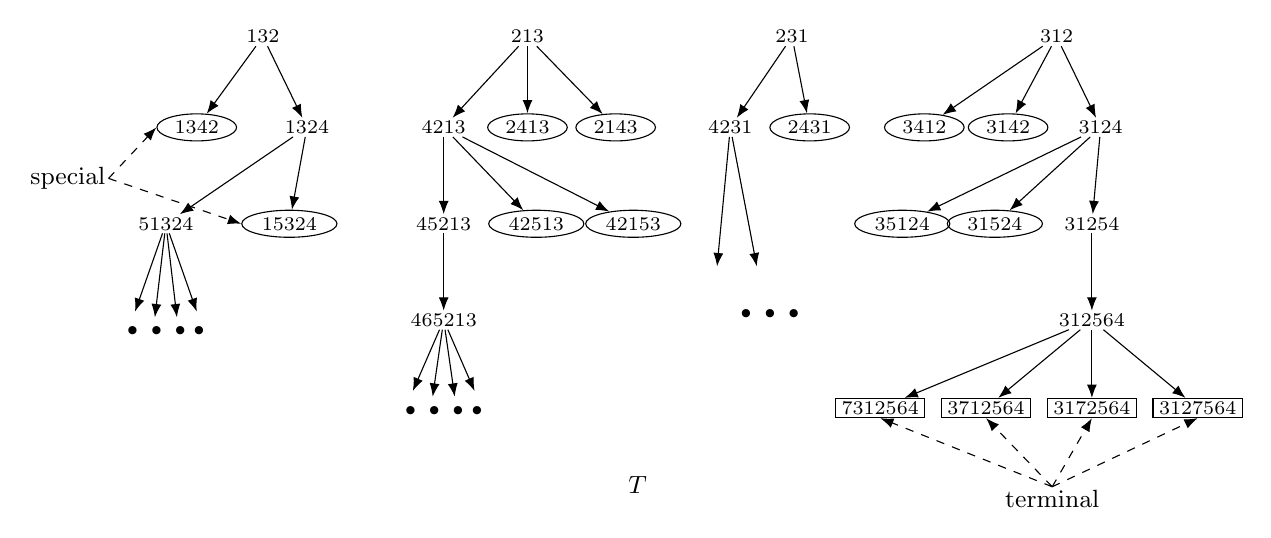
\begin{tikzpicture}[
  x=0.56cm,
  y=0.72cm,
  >=Latex,
  every node/.style={font=\scriptsize,inner sep=1pt},
  circ/.style={draw,ellipse,inner xsep=2.2pt,inner ysep=1.2pt},
  terminal/.style={draw,rectangle,inner xsep=2.2pt,inner ysep=1.2pt},
  edge/.style={->,thin},
  callout/.style={->,dashed,thin}
]
% Roots
\node (r132) at (0,7.0) {$132$};
\node (r213) at (6,7.0) {$213$};
\node (r231) at (12,7.0) {$231$};
\node (r312) at (18,7.0) {$312$};

% Second level
\node[circ] (n1342) at (-1.5,5.4) {$1342$};
\node (n1324) at (1.0,5.4) {$1324$};
\node (n4213) at (4.1,5.4) {$4213$};
\node[circ] (n2413) at (6.0,5.4) {$2413$};
\node[circ] (n2143) at (8.0,5.4) {$2143$};
\node (n4231) at (10.6,5.4) {$4231$};
\node[circ] (n2431) at (12.4,5.4) {$2431$};
\node[circ] (n3412) at (15.0,5.4) {$3412$};
\node[circ] (n3142) at (16.9,5.4) {$3142$};
\node (n3124) at (19.0,5.4) {$3124$};

\draw[edge] (r132) -- (n1342);
\draw[edge] (r132) -- (n1324);
\draw[edge] (r213) -- (n4213);
\draw[edge] (r213) -- (n2413);
\draw[edge] (r213) -- (n2143);
\draw[edge] (r231) -- (n4231);
\draw[edge] (r231) -- (n2431);
\draw[edge] (r312) -- (n3412);
\draw[edge] (r312) -- (n3142);
\draw[edge] (r312) -- (n3124);

% Third level
\node (n51324) at (-2.2,3.7) {$51324$};
\node[circ] (n15324) at (0.6,3.7) {$15324$};
\node (n45213) at (4.1,3.7) {$45213$};
\node[circ] (n42513) at (6.2,3.7) {$42513$};
\node[circ] (n42153) at (8.4,3.7) {$42153$};
\node[circ] (n35124) at (14.5,3.7) {$35124$};
\node[circ] (n31524) at (16.6,3.7) {$31524$};
\node (n31254) at (18.8,3.7) {$31254$};

\draw[edge] (n1324) -- (n51324);
\draw[edge] (n1324) -- (n15324);
\draw[edge] (n4213) -- (n45213);
\draw[edge] (n4213) -- (n42513);
\draw[edge] (n4213) -- (n42153);
\draw[edge] (n3124) -- (n35124);
\draw[edge] (n3124) -- (n31524);
\draw[edge] (n3124) -- (n31254);

% Special callout
\node[anchor=east,font=\small] (special) at (-3.5,4.5) {special};
\draw[callout] (special.east) -- (n1342.west);
\draw[callout] (special.east) -- (n15324.west);

% Continuing branches
\node (dots51324) at (-2.2,1.8) {$\bullet\ \bullet\ \bullet\ \bullet$};
\draw[edge] (n51324) -- ++(-0.7,-1.55);
\draw[edge] (n51324) -- ++(-0.25,-1.65);
\draw[edge] (n51324) -- ++(0.25,-1.65);
\draw[edge] (n51324) -- ++(0.7,-1.55);

\node (n465213) at (4.1,2.0) {$465213$};
\draw[edge] (n45213) -- (n465213);
\node (dots465213) at (4.1,0.4) {$\bullet\ \bullet\ \bullet\ \bullet$};
\draw[edge] (n465213) -- ++(-0.7,-1.25);
\draw[edge] (n465213) -- ++(-0.25,-1.35);
\draw[edge] (n465213) -- ++(0.25,-1.35);
\draw[edge] (n465213) -- ++(0.7,-1.25);

\node (dots4231) at (11.5,2.1) {$\bullet\ \bullet\ \bullet$};
\draw[edge] (n4231) -- ++(-0.3,-2.45);
\draw[edge] (n4231) -- ++(0.6,-2.45);

\node (n312564) at (18.8,2.0) {$312564$};
\draw[edge] (n31254) -- (n312564);

% Terminal vertices
\node[terminal] (t1) at (14.0,0.45) {$7312564$};
\node[terminal] (t2) at (16.4,0.45) {$3712564$};
\node[terminal] (t3) at (18.8,0.45) {$3172564$};
\node[terminal] (t4) at (21.2,0.45) {$3127564$};
\draw[edge] (n312564) -- (t1);
\draw[edge] (n312564) -- (t2);
\draw[edge] (n312564) -- (t3);
\draw[edge] (n312564) -- (t4);

\node[font=\small] (terminal-label) at (17.9,-1.15) {terminal};
\draw[callout] (terminal-label.north) -- (t1.south);
\draw[callout] (terminal-label.north) -- (t2.south);
\draw[callout] (terminal-label.north) -- (t3.south);
\draw[callout] (terminal-label.north) -- (t4.south);

\node[font=\small] at (8.5,-0.9) {$T$};
\end{tikzpicture}
\caption{A portion of the directed tree $T$.}
\label{fig:tree}
\end{figure}

To complete the proof, we make the following observation. As we adjoin
consecutive integers, starting with $A^*\in\Mcal(3)$, to form a
permutation $P$ of $\Zpos$, we move in the obvious way along a directed
path in the tree. Suppose we reach a special vertex
$A=a_1\ldots a_n$. By definition, the block of $A$ spanned by
$\{1,2,3\}$ contains a subsequence $a_{i_1}a_{i_2}a_{i_3}$ which is a
permutation of $\{a,a+d,a+2d\}\ne\{1,2,3\}$. If we restrict our attention
from now on to just those integers of the form $a+md$, $m\ge0$, then we
can move back to the appropriate root of $T$, i.e., the permutation of
$\{1,2,3\}$ having the same relative order as
$a_{i_1}a_{i_2}a_{i_3}$. Since $T$ is finite, as we form $P$ we must pass
through the roots of $T$ an unbounded number of times. However, this
implies that in $P$ some pair of integers in $\{1,2,3\}$ must have an
unbounded number of integers separating them. This contradicts the
definition of a permutation of $\Zpos$, and the proof is complete.
\end{proof}

The additional freedom allowed by doubly-infinite permutations can be
used to prevent the occurrence of monotone 4-term A.P.s.

\fact{6}
\[
 \Dcal_4\ne\varnothing.
\]

\begin{proof}
Define the blocks $B_i$, $i\ge0$, as follows:
\[
 \begin{aligned}
 B_0&=1,\\
 B_{2i+1}&=(2B_{2i})'(2B_{2i}+1)',\\
 B_{2i+2}&=(2B_{2i+1}+1)'(2B_{2i+1})',\qquad i\ge0,
 \end{aligned}
\]
where $B'$ denotes the block $B$ written in reverse order. Define the
doubly-infinite permutation $P$ of $\Zpos$ by
\[
 \begin{aligned}
 P&=\ldots B_4B_2B_0B_1B_3\ldots\\
  &=\ldots,28,20,24,16,7,5,6,4,1,2,3,8,12,10,14,9,13,11,15,\ldots.
 \end{aligned}
\]
We claim that $P\in\Dcal_4$.

We first note that for all $i\ge0$, $B_i$ is a permutation of
$[2^i,2^{i+1}-1]$ containing no monotone 3-term A.P. Suppose now that $P$
contains a monotone 4-term A.P. $X=\{x,y,z,w\}$ with either
$x>y>z>w$ or $x<y<z<w$, where we have chosen $X$ so that
$d=|x-y|$ is minimal. There are several possibilities.

\begin{enumerate}[label=(\roman*),leftmargin=2.3em]
\item The smallest two elements of $X$ belong to the same block $B_i$.
Then $d<2^i$, so the largest two elements of $X$ are in $B_{i+1}$.
Consequently, $x,y,z,w$ all have the same parity. If $2j+1$ and $2k+1$
are in $B_i$, then $2j$ and $2k$ are also in $B_i$ with the same relative
order. Hence, we may assume $x,y,z,w$ are all even. But then
\[
 \frac12X=\left\{\frac{x}{2},\frac{y}{2},\frac{z}{2},\frac{w}{2}\right\}
\]
is a monotone 4-term A.P. in $P$: the smallest two elements of
$\tfrac12X$ appear in $B_{i-1}$ in reverse order of their appearance in
$B_i$, the largest two appear in $B_i$ in reverse order of their
appearance in $B_{i+1}$, and the order of $B_i$ and $B_{i-1}$ in $P$ is
the reverse of that of $B_{i+1}$ and $B_i$. This contradicts the
minimality of $d$.

\item Suppose $y$ and $z$ occur in the same block $B_i$. Then the largest
element of $X$ occurs in $B_{i+1}$ and the smallest occurs in $B_j$ for
some $j<i$. But this requires $B_i$ to appear between $B_{i+1}$ and $B_j$
in $P$, which is impossible.

\item Suppose the largest two elements of $X$ occur in the same block
$B_i$. The third largest element of $X$ must be at least $2^{i-1}$.
Otherwise, because the second largest element is at least $2^i$, we would
have $d>2^{i-1}$, forcing the smallest element of $X$ to be negative.
Thus, the third largest element of $X$ is in $B_{i-1}$. Hence, by (i), the
smallest element of $X$ is in $B_j$ for some $j<i-1$. As before, this
requires $B_{i-1}$ to appear between $B_j$ and $B_i$ in $P$, which is
impossible.

\item Suppose each element of $X$ belongs to a different block $B_i$ of
$P$. Let $B_i$ denote the block containing the largest element of $X$.
Then we may argue as in (ii) and (iii) that the second largest element of
$X$ is not contained in $B_{i-1}$. Consequently, $d>2^{i-1}$, so the
third largest element of $X$ must be negative, a contradiction.
\end{enumerate}
Since the construction of the $B_i$ prohibits the occurrence of three
elements of $X$ in a single block, we have proved that $P$ has no
monotone 4-term A.P.
\end{proof}

\medskip
\noindent\textbf{Concluding remarks.}
There are a number of questions which we were either unable to resolve or
did not have a chance to look at. We mention a few of these.

\begin{enumerate}[leftmargin=2.2em]
\item The most natural question remaining is whether or not
$\Scal_4=\varnothing$; i.e., whether or not every singly-infinite
permutation of $\Zpos$ contains a monotone 4-term A.P. It is not clear at
present in which direction the truth lies.

\item The following modular analogue to the finite problem has been
studied by M. Nathanson [3]. A subsequence
$a_{i_0},\ldots,a_{i_{t-1}}$ of a permutation $a_1a_2\ldots a_n$ of
$[1,n]$ is called a monotone A.P. modulo $n$ if, for some $a$ and
$d\ne0$,
\[
 a_{i_k}\equiv a+kd\pmod n,\qquad 0\le k<t.
\]
Nathanson has shown (see [3]) that:
\begin{enumerate}[label=(\roman*),leftmargin=2.3em]
\item If $n\ne2^r$, then any permutation of $[1,n]$ contains a monotone
3-term A.P. modulo $n$.
\item If $n=2^r$, then there is a permutation of $[1,n]$ which contains
no monotone 3-term A.P.
\end{enumerate}
On the other hand, it is easily seen that a permutation of $[1,n]$ which
contains no monotone 3-term A.P. also contains no monotone 5-term A.P.
modulo $n$. As in the preceding question, the situation for 4-term A.P.s
modulo $n$ is unclear.

\item It is possible to partition $\Zpos$ into three sets, each of which
can be permuted so as to have no monotone 3-term A.P. For example, define
the partition of $\Zpos$ into consecutive intervals $A_k$ by
\[
 A_1=[1,100],
 \qquad
 |A_{k+1}|=\left\lfloor\frac32|A_k|\right\rfloor,
 \qquad k\ge1.
\]
Now rearrange each $A_k$ into $A_k^*$ containing no monotone 3-term A.P.,
and define
\[
 \begin{aligned}
 \mathscr A&=A_1^*A_4^*A_7^*A_{10}^*\ldots,\\
 \mathscr B&=A_2^*A_5^*A_8^*A_{11}^*\ldots,\\
 \mathscr C&=A_3^*A_6^*A_9^*A_{12}^*\ldots.
 \end{aligned}
\]
It is easily checked that $\mathscr A$, $\mathscr B$, and $\mathscr C$
form the desired partition. Whether this can be done for some partition
of $\Zpos$ into two sets is not known.

\item Let $\mathscr A$ denote the set of all infinite subsets $A$ of
$\Zpos$ for which there exists a singly-infinite permutation of $A$
having no monotone 3-term A.P. What is
\[
 \sup_{A\in\mathscr A}\liminf_{n\to\infty}
 \frac{|A\cap[1,n]|}{n}\,?
\]
What is
\[
 \sup_{A\in\mathscr A}\limsup_{n\to\infty}
 \frac{|A\cap[1,n]|}{n}\,?
\]

\item The preceding questions could also be asked for $\mathbb Z$, the
set of all integers. Only preliminary results are known for this case.
For example, using Fact 4, it is easy to construct permutations of
$\mathbb Z$ which have no monotone 7-term A.P.
\end{enumerate}

\section*{References}
\begin{enumerate}[label={[\arabic*]},leftmargin=2.6em,itemsep=0pt]
\item R. C. Entringer and D. E. Jackson, \emph{Elementary Problem 2440},
Amer. Math. Monthly \textbf{80} (1973), p.~1058.
\item J. H. Folkman (unpublished).
\item M. B. Nathanson, \emph{Permutations, periodicity and chaos},
Journ. Comb. Th. (A) \textbf{22} (1977), pp.~61--68.
\item Tom Odda, \emph{Solution to Problem E 2440}, Amer. Math. Monthly
\textbf{82} (1975), p.~74.
\item G. J. Simmons, \emph{Solution to Problem E 2440}, ibid.
\textbf{82} (1975), pp.~76--77.
\item H. E. Thomas Jr., \emph{Solution to Problem E 2440}, ibid.
\textbf{82} (1975), pp.~75--76.
\end{enumerate}

\bigskip
\begin{center}
\emph{Received on 29 June 1976}
\end{center}

\end{document}
